% !TEX encoding = UTF-8 Unicode
%%%%%%%%%%%%%%%%%%%%%%%%%%%%%%%%%%%%%%%%%
% Beamer Presentation
% LaTeX Template
% Version 1.0 (10/11/12)
%
% This template has been downloaded from:
% http://www.LaTeXTemplates.com
%
% License:
% CC BY-NC-SA 3.0 (http://creativecommons.org/licenses/by-nc-sa/3.0/)
%
%%%%%%%%%%%%%%%%%%%%%%%%%%%%%%%%%%%%%%%%%

%----------------------------------------------------------------------------------------
%	PACKAGES AND THEMES
%----------------------------------------------------------------------------------------

\documentclass{beamer}

\mode<presentation> {

% The Beamer class comes with a number of default slide themes
% which change the colors and layouts of slides. Below this is a list
% of all the themes, uncomment each in turn to see what they look like.

%\usetheme{default}
%\usetheme{AnnArbor}
%\usetheme{Antibes}
%\usetheme{Bergen}
%\usetheme{Berkeley}
%\usetheme{Berlin}
%\usetheme{Boadilla}
%\usetheme{CambridgeUS}
%\usetheme{Copenhagen}
%\usetheme{Darmstadt}
%\usetheme{Dresden}
%\usetheme{Frankfurt}
%\usetheme{Goettingen}
%\usetheme{Hannover}
%\usetheme{Ilmenau}
%\usetheme{JuanLesPins}
%\usetheme{Luebeck}
%\usetheme{Madrid}
%\usetheme{Malmoe}
%\usetheme{Marburg}
%\usetheme{Montpellier}
%\usetheme{PaloAlto}
%\usetheme{Pittsburgh}
%\usetheme{Rochester}
\usetheme{Singapore}
%\usetheme{Szeged}
%\usetheme{Warsaw}

% As well as themes, the Beamer class has a number of color themes
% for any slide theme. Uncomment each of these in turn to see how it
% changes the colors of your current slide theme.

%\usecolortheme{albatross}
%\usecolortheme{beaver}
%\usecolortheme{beetle}
%\usecolortheme{crane}
%\usecolortheme{dolphin}
%\usecolortheme{dove}
%\usecolortheme{fly}
%\usecolortheme{lily}
%\usecolortheme{orchid}
%\usecolortheme{rose}
%\usecolortheme{seagull}
%\usecolortheme{seahorse}
%\usecolortheme{whale}
%\usecolortheme{wolverine}

%\setbeamertemplate{footline} % To remove the footer line in all slides uncomment this line
%\setbeamertemplate{footline}[page number] % To replace the footer line in all slides with a simple slide count uncomment this line

%\setbeamertemplate{navigation symbols}{} % To remove the navigation symbols from the bottom of all slides uncomment this line
}

\usepackage{graphicx} % Allows including images
\usepackage{booktabs} % Allows the use of \toprule, \midrule and \bottomrule in tables
\usepackage{xeCJK}
\setCJKmainfont{SourceHanSerif-Regular}
\usepackage{color}
\usepackage{listings}
\lstset{numbers=left}
\usepackage{fancyvrb}%use Verbatim-the extended verbatim
\usepackage{tikz}


%----------------------------------------------------------------------------------------
%	TITLE PAGE
%----------------------------------------------------------------------------------------

\title[Django]{python} % The short title appears at the bottom of every slide, the full title is only on the title page
\subtitle{function}
\author{} % Your name
\institute[计算机科学与技术学院] % Your institution as it will appear on the bottom of every slide, may be shorthand to save space
{
贵州大学 \\ % Your institution for the title page
\medskip
\textit{hnzhang1@gzu.edu.cn} % Your email address
}
\date{\today} % Date, can be changed to a custom date

\begin{document}

\begin{frame}
\titlepage % Print the title page as the first slide
\end{frame}
\begin{frame}{Overview}
\tableofcontents
\end{frame}
%\begin{Verbatim}[numbers=left,frame=single,rulecolor=\color{red}]

%\end{Verbatim}



%\begin{columns}
%\column{2.8cm}{if}
%\column{2.8cm}{if-else}
%\column{3.1cm}{if-elif}
%\begin{Verbatim}[numbers=none,frame=single,rulecolor=\color{red}]
%\column{3.1cm}{if-elif-else}
%\end{columns}
\section{introduce of function}
\begin{frame}{introduce of function}
函数(方法)具有以下特点:
\begin{itemize}
\item 是一段代码
\item 能完成特定功能
\item 可以在其他地方被调用
\item 可以接收参数或不接收参数
\item 可以有返回值或没有返回值
\end{itemize}
函数用于将一个\textcolor{red}{复杂}的问题\textcolor{red}{分解}为若干个\textcolor{red}{简单}的子问题。
\end{frame}
\begin{frame}{函数的类别}
\begin{description}
\item[ 内建函数 ]  int()、chr()、ord()、round()等
\item[ 自定义函数 ] 
\end{description}

\end{frame}
\section{define a function}
\begin{frame}[fragile]{函数的定义}
\begin{Verbatim}[numbers=left,frame=single,rulecolor=\color{red}]
def functionName(parameter1, parameter2, …):
    functionBlock
    return aValue
\end{Verbatim}
第1行称为函数签名,用于指定函数名称以及函数的每个形式参数变量名,注意要有结尾的英文冒号。
\begin{description}
\item[ def ] 定义函数的关键字
\item[ functionName ] 函数名
\item[ parameter1…] 参数\footnote{函数可以不需要参数}
\item[ functionBlock ] 函数体
\item[ return ] 表明此函数是有返回值的\footnote{函数可以不返回任何值}
\item[ aValue ] 函数的返回值
\end{description}

\end{frame}

\begin{frame}[fragile]{函数的调用}
\begin{columns}
\column{.8\textwidth}
\begin{Verbatim}[numbers=left,frame=single,rulecolor=\color{red}]
import math

def myGCD(a,b):
    c, d = a, b
    while a % b != 0:
        a, b = b, a % b
    print(c,'和',d,'的最大公约数是:',b)

a = int(input("a:"))
b = int(input("b:"))
myGCD(a,b)
print(math.gcd(a, b))
\end{Verbatim}
\column{.2\textwidth}
\begin{Verbatim}[numbers=none,frame=single,rulecolor=\color{blue}]
一系列的
import

一系列的
函数定义



任意数量的
全局代码

程序的主体
\end{Verbatim}

\end{columns}
\end{frame}

\begin{frame}[fragile]{默认(可选)参数}
\begin{columns}
\column{.11\textwidth}

{\tiny 可以给一个参数指定默认值(\textcolor{red}{在函数签名中为参数赋值}),这样的参数也叫可选参数。可选参数可以有多个,但所有的\textcolor{red}{可选参数都要定义在必选参数之后}。}
\column{.89\textwidth}
\begin{Verbatim}[numbers=right,frame=single,rulecolor=\color{red}]
def is_prime(first_n=10):
    prime_list = [2]
    i = 3
    while True:
        for d in range(2, i):
            if i % d == 0:
                break
            elif (i % d != 0) and (d == (i-1)):
                prime_list.append(i)
        if len(prime_list) == first_n:
            break
        i += 1
    return prime_list

print(is_prime())
print(is_prime(5))
\end{Verbatim}

\end{columns}
\end{frame}


\begin{frame}[fragile]{多态性}
\begin{columns}
\column{.5\textwidth}
\begin{Verbatim}[numbers=left,frame=single,rulecolor=\color{red}]
import math

def my_power(a, b):
    return a**b
    
n1 = my_power(2,5)
n2 = my_power(math.pi, 1)
print(n1, n2)


32 3.141592653589793
\end{Verbatim}
\column{.5\textwidth}
从\textit{my\_power()}这个函数的返回值可以看出,传递int值的时候,返回的也是int值;如果传递的是浮点类型的值,返回值就是浮点类型的。

\textit{python}的这个特性体现了其灵活性,即多态性。\textcolor{red}{多态性允许定义一个函数,供不同类型的对象使用。}

但是要注意传递恰当类型的对象,如果向\textit{my\_power()}函数传递字符串类型的对象的话,程序会产生\textit{TypeError}错误。
\end{columns}
\end{frame}


\begin{frame}[fragile]{返回多个值}
\begin{columns}
\column{.8\textwidth}
\begin{Verbatim}[numbers=left,frame=single,rulecolor=\color{red}]
import math

def move(x, y, distance, angle = 0):
    new_x = x + distance * math.cos(angle)
    new_y = y + distance * math.sin(angle)
    return new_x, new_y
    
x, y = move(0, 0, 1.414, math.pi/4)
print(x, y)
z = move(0, 0, 2, math.pi/6)
print(z)

0.9998489885977783 0.999848988597778
(1.7320508075688774, 0.9999999999999999)
\end{Verbatim}
\column{.2\textwidth}
 
 
 
 
 
 
 
 
 
 
第8行形式上返回了\textcolor{red}{两个值},通过
第10可以看出\textcolor{red}{其实是一个元组}。


\end{columns}
\end{frame}

\begin{frame}[fragile]{列表解析}
当想要对一个序列中的每个元素都执行某个特定的操作时,通常可以使用\textit{for}循环来实现。
在\textit{python}中,可以使用\textcolor{red}{列表解析}。
\begin{Verbatim}[numbers=left,frame=single,rulecolor=\color{red}]
import math

l = [2, 3, 4]
m = [pow(x, 2) for x in l]
n = [math.sqrt(y) for y in m]
print(m)
print(n)

[4, 9, 16]
[2.0, 3.0, 4.0]
\end{Verbatim}

\end{frame}


\begin{frame}[fragile]{向函数传递不可变对象\footnote{\url{https://www.python-course.eu/passing_arguments.php}}}
\begin{columns}
\column{.77\textwidth}
\begin{Verbatim}[numbers=left,frame=single,rulecolor=\color{red}]
def double(l):
    print('before:: l=',l,'id(l)=',id(l))
    l = l * 2
    print('after:: l=',l,'id(l)=',id(l))

x = 5
print('x=',x,'id(x)=:', id(x))
double(x)
print('x=',x)

x= 5 id(x)=: 4385389696
before:: l= 5 id(l)= 4385389696
after:: l= 10 id(l)= 4385389856
x= 5
\end{Verbatim}
\column{.23\textwidth}
\begin{block}{before \textit{line3}}
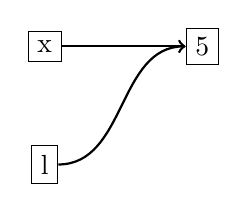
\begin{tikzpicture}
%\draw [thick,red,dashed,above] (0,0) rectangle (3,5) node{host A};
\node [draw,rectangle] (x) at(0,4.5){x};
\node [draw,rectangle] (xv) at(2,4.5){5};

\node [draw,rectangle] (lx) at(0,3){l};
%\node [draw,rectangle] (lxv) at(2,3){10};

\draw[thick,->](x) to[out=0,in=180] (xv);
\draw[thick,->](lx) to[out=0,in=180] (xv);
%\draw[thick,->](lx) to[out=0,in=180] (lxv);

%\draw[thick,->](p) to[out=0,in=180] (o);


\end{tikzpicture}
\end{block}
\begin{block}{after \textit{line3}}
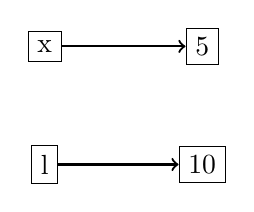
\begin{tikzpicture}
\node [draw,rectangle] (x) at(0,4.5){x};
\node [draw,rectangle] (xv) at(2,4.5){5};

\node [draw,rectangle] (lx) at(0,3){l};
\node [draw,rectangle] (lxv) at(2,3){10};

\draw[thick,->](x) to[out=0,in=180] (xv);
\draw[thick,->](lx) to[out=0,in=180] (lxv);
\end{tikzpicture}
\end{block}

\end{columns}
\end{frame}

\begin{frame}[fragile]{向函数传递可变对象\textit{I}}
\begin{columns}
\column{.77\textwidth}
\begin{Verbatim}[numbers=left,frame=single,rulecolor=\color{red}]
def double(f):
    print('before:: f=',f,'id(f)=',id(f))
    f = f * 2
    print('after:: f=',f,'id(f)=',id(f))

l = [2, 3, 4]
print('l=',l,'id(l)=:', id(l))
double(l)
print('l:', l)

l= [2, 3, 4] id(l)=: 4386889608
before:: f= [2, 3, 4] id(f)= 4386889608
after:: f= [2, 3, 4, 2, 3, 4] 
id(f)= 4388025352
l: [2, 3, 4]
\end{Verbatim}
\column{.23\textwidth}
\begin{block}{before \textit{line3}}
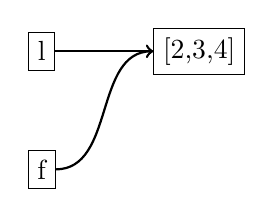
\begin{tikzpicture}
%\draw [thick,red,dashed,above] (0,0) rectangle (3,5) node{host A};
\node [draw,rectangle] (x) at(0,4.5){l};
\node [draw,rectangle] (xv) at(2,4.5){[2,3,4]};

\node [draw,rectangle] (lx) at(0,3){f};
%\node [draw,rectangle] (lxv) at(2,3){10};

\draw[thick,->](x) to[out=0,in=180] (xv);
\draw[thick,->](lx) to[out=0,in=180] (xv);
%\draw[thick,->](lx) to[out=0,in=180] (lxv);

%\draw[thick,->](p) to[out=0,in=180] (o);


\end{tikzpicture}
\end{block}
\begin{block}{after \textit{line3}}
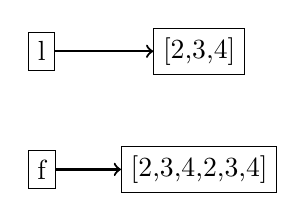
\begin{tikzpicture}
\node [draw,rectangle] (x) at(0,4.5){l};
\node [draw,rectangle] (xv) at(2,4.5){[2,3,4]};

\node [draw,rectangle] (lx) at(0,3){f};
\node [draw,rectangle] (lxv) at(2,3){[2,3,4,2,3,4]};

\draw[thick,->](x) to[out=0,in=180] (xv);
\draw[thick,->](lx) to[out=0,in=180] (lxv);
\end{tikzpicture}
\end{block}

\end{columns}
\end{frame}

\begin{frame}[fragile]{向函数传递可变对象\textit{II}\footnote{Side effects: A function is said to have a side effect if, in addition to producing a value, it modifies the caller's environment in other ways. }}
\begin{columns}
\column{.77\textwidth}
\begin{Verbatim}[numbers=left,frame=single,rulecolor=\color{red}]
def double_2(f):
    print('before:: f=',f,'id(f)=',id(f))
    del f[-1]
    print('after:: f=',f,'id(f)=',id(f))

l = [2, 3, 4]
print('l=',l,'id(l)=',id(l))
double_2(l)
print('l:', l)

l= [2, 3, 4] id(l)= 4377313160
before:: f= [2, 3, 4] id(f)= 4377313160
after:: f= [2, 3] id(f)= 4377313160
l: [2, 3]
\end{Verbatim}
\column{.23\textwidth}
\begin{block}{before \textit{line3}}
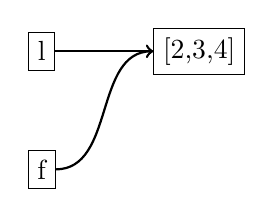
\begin{tikzpicture}
%\draw [thick,red,dashed,above] (0,0) rectangle (3,5) node{host A};
\node [draw,rectangle] (x) at(0,4.5){l};
\node [draw,rectangle] (xv) at(2,4.5){[2,3,4]};

\node [draw,rectangle] (lx) at(0,3){f};
%\node [draw,rectangle] (lxv) at(2,3){10};

\draw[thick,->](x) to[out=0,in=180] (xv);
\draw[thick,->](lx) to[out=0,in=180] (xv);
%\draw[thick,->](lx) to[out=0,in=180] (lxv);

%\draw[thick,->](p) to[out=0,in=180] (o);


\end{tikzpicture}
\end{block}
\begin{block}{after \textit{line3}}
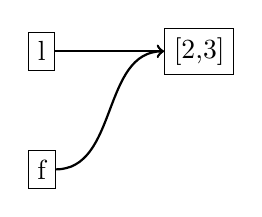
\begin{tikzpicture}
\node [draw,rectangle] (x) at(0,4.5){l};
\node [draw,rectangle] (xv) at(2,4.5){[2,3]};

\node [draw,rectangle] (lx) at(0,3){f};
%\node [draw,rectangle] (lxv) at(2,3){[2,3,4,2]};

\draw[thick,->](x) to[out=0,in=180] (xv);
\draw[thick,->](lx) to[out=0,in=180] (xv);
\end{tikzpicture}
\end{block}

\end{columns}
\end{frame}

\begin{frame}[fragile]{如何避免函数改变主程序中变量的值}
\begin{columns}
\column{.77\textwidth}
\begin{Verbatim}[numbers=left,frame=single,rulecolor=\color{red}]
def double_2(f):
    print('before:: f=',f,'id(f)=',id(f))
    del f[-1]
    print('after:: f=',f,'id(f)=',id(f))

l = [2, 3, 4]
print('l=',l,'id(l)=',id(l))
double_2(l[:])
print('l:', l)

l= [2, 3, 4] id(l)= 4537892744
before:: f= [2, 3, 4] id(f)= 4539028552
after:: f= [2, 3] id(f)= 4539028552
l: [2, 3, 4]
\end{Verbatim}
\column{.23\textwidth}
\begin{block}{before \textit{line3}}
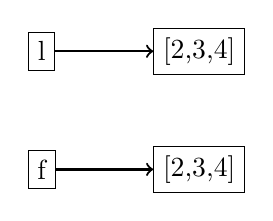
\begin{tikzpicture}
%\draw [thick,red,dashed,above] (0,0) rectangle (3,5) node{host A};
\node [draw,rectangle] (x) at(0,4.5){l};
\node [draw,rectangle] (xv) at(2,4.5){[2,3,4]};

\node [draw,rectangle] (lx) at(0,3){f};
\node [draw,rectangle] (lxv) at(2,3){[2,3,4]};

\draw[thick,->](x) to[out=0,in=180] (xv);
\draw[thick,->](lx) to[out=0,in=180] (lxv);
%\draw[thick,->](lx) to[out=0,in=180] (lxv);

%\draw[thick,->](p) to[out=0,in=180] (o);


\end{tikzpicture}
\end{block}
\begin{block}{after \textit{line3}}
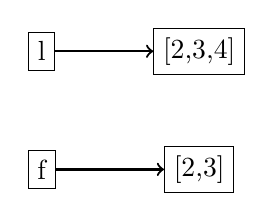
\begin{tikzpicture}
\node [draw,rectangle] (x) at(0,4.5){l};
\node [draw,rectangle] (xv) at(2,4.5){[2,3,4]};

\node [draw,rectangle] (lx) at(0,3){f};
\node [draw,rectangle] (lxv) at(2,3){[2,3]};

\draw[thick,->](x) to[out=0,in=180] (xv);
\draw[thick,->](lx) to[out=0,in=180] (lxv);
\end{tikzpicture}
\end{block}

\end{columns}
\end{frame}
\begin{frame}{lamda}
\end{frame}
\section{module}
\begin{frame}{模块}
\end{frame}

%----------------------------------------------------------------------------------------
%	PRESENTATION SLIDES
%----------------------------------------------------------------------------------------
\section{homework}
\begin{frame}{Homework}
\begin{enumerate}
\item
求出前10个素数\footnote{质数(prime number)又称素数,有无限个。质数定义为在大于1的自然数中,除了1和它本身以外不再有其他因数。}。
\item
使用辗转相除法\footnote{用较大数除以较小数,再用出现的余数(第一余数)去除除数,再用出现的余数(第二余数)去除第一余数,如此反复,直到最后余数是0为止。如果是求两个数的最大公约数,那么最后的除数就是这两个数的最大公约数。}求任意两个数的最大公约数。
%\item
%找零钱。输入收费金额和客户所付的钱,给出需要怎么找零。要求找零的钱币张数最少。(即需要多少1元的,多少2元的,多少5元的等)
\end{enumerate}
\end{frame}
\section{Q\&A}
\begin{frame}
\center{\Huge{Q\&A}}
\end{frame}


%How do I uninstall?
%
%	1.	Remove /Applications/Wireshark.app
%	2.	Remove /Library/Application Support/Wireshark
%	3.	Remove the wrapper scripts from /usr/local/bin
%	4.	Unload the org.wireshark.ChmodBPF.plist launchd job
%	5.	Remove /Library/LaunchDaemons/org.wireshark.ChmodBPF.plist
%	6.	Remove the access_bpf group.
%	7.	Remove /etc/paths.d/Wireshark
%	8.	Remove /etc/manpaths.d/Wireshark
\end{document} 

